\chapter{Indexácia $k$-nadslova}

V predošlej kapitole sme si popísali, ako vieme nájsť $k$-nadslovo k nejakej
množine reťazcov. V tejto kapitole si popíšeme rôzne typy dotazov, ktoré
vieme implementovať s pomocou nájdeného $k$-nadslova.

Spomenuté typy dotazov sú určené primárne na zisťovanie
rôznych vlastností sady čítaní, preto množinu vstupných reťazcov budeme 
nazývať \emph{čítania}. Pripomíname, že všetky dotazy budú zisťovať nejakú
informáciu o podreťazcoch, ktoré sú dlhé práve $k$.

\section{Prítomnosť podreťazca}

Úplne najzákladnejšou otázkou, na ktorú chceme vedieť odpovedať, je prítomnosť
nejakého podreťazca dĺžky presne $k$ vo vstupných čítaniach. Ako sa neskôr ukáže,
vedieť odpovedať na takýto dotaz nám pomôže vybudovať dodatočné podporné
štruktúry, pomocou ktorých budeme vedieť odpovedať aj na zložitejšie dotazy.

Ako prvé je dôležité všimnúť si, že prítomnosť nejakého reťazca v $k$-nadslove
nám nezaručuje, že sa vyskytoval aj v nejakom z pôvodných čítaní. Vezmime si
napríklad $k = 4$ a dve čítania, \texttt{ACGA} a \texttt{ACGT}. Ich $k$-nadslovom
môže byť napríklad reťazec \texttt{ACGACGT}, ktorý síce obsahuje aj
podreťazec \texttt{CGAC}, no ten sa nevyskytuje ani v jednom z pôvodných čítaní.

Pre tento účel mierne modifikujeme algoritmus na hľadanie $k$-nadslova tak, aby nám
vedel pre každý znak výsledného $k$-nadslova povedať, či sa ním končí nejaká $k$-tica,
ktorá sa vyskytuje v niektorom pôvodnom čítaní. To docielime jednoducho tak, že
pre každú hranu, ktorú budeme mať v našom grafe, si zapamätáme, či reprezentuje
nutnú hranu, inými slovami povedané, či sa $k$-tica, ktorú reprezentuje, vyskytuje
v niektorom zo vstupných čítaní.

Pri prepisovaní sledu na konkrétny reťazec si budeme zároveň vytvárať pole
pravdivostných hodnôt, do ktorého pre každý znak, ktorý pripisujeme na koniec
generovaného $k$-nadslova, uložíme hodnotu $Pravda$, ak práve pridávaný znak
prichádza z nutnej hrany. Prvých $k-1$ znakov, preklad prvého vrchola, dostane
hodnotu $Pravda$, keďže každý vrchol predstavuje $k-1$-ticu znakov, ktorá sa
nachádzala v niektorom vstupnom slove. Toto pole budeme nazývať \emph{poľom výskytov}.

Nakoniec potrebujeme pre každý dotazovaný podreťazec určiť, kde sa nachádza v $k$-nadslove.
Pre tento účel využijeme štruktúru FM-index \cite{fm_index}, konkrétne jeho implementáciu
z knižnice SDSL \cite{sdsl}. Pomocou FM-indexu vieme zistiť, kde sa začínajú všetky
výskyty nejakého podreťazca v $k$-nadslove v čase priamo úmernom súčtu dĺžky vyhľadávaného podreťazca
a počtu výskytov. Napriek tomu zaberá pri dĺžke uloženého slova $m$ zhruba $m/2$
bajtov.

Na dotazovaný reťazec $r$ teda nájdeme všetky jeho začiatky v $k$-nadslove. Ak
v poli výskytov nájdeme aspoň pre jeden koniec výskytu hodnotu $Pravda$, odpovieme
tiež $Pravda$, v opačnom prípade odpovieme $Nepravda$.

Aby sme čo najviac zmenšili veľkosť poľa výskytov, uložíme si ho skomprimované
podľa techniky z článku Ramana, Ramana a Raa \cite{rrr_vector}. Takto zostrojené pole
dĺžky $m$ s $n$ nastavenými bitmi má veľkosť $\beta(n, m) + o(n) + O(log log n)$ bitov,
kde $\beta(n, m)$ je dolné teoretické obmedzenie na počet bitov potrebných na reprezentáciu
$n$-prvkovej podmnožiny z $m$-prvkovej množiny, zároveň však vie zisťovať hodnotu na danej
pozícii v konštantnom čase. Používame implementáciu z SDSL.

\section{Počet výskytov podreťazca}
\label{sekcia:index_pocet}

Podobne ako zisťovanie prítomnosti nejakého podreťazca môžeme vyriešiť aj podporu
pre dotazy, koľkokrát sa daný podreťazec nachádza v zadaných čítaniach. Jediný rozdiel
bude v tom, že si pre každú nutnú hranu budeme pamätať, koľkokrát sa vyskytovala jej
zodpovedajúca $k$-tica písmen v čítaniach; pre nepovinné hrany si budeme pamätať nulu.

Podobne ako pri dotazoch na prítomnosť si pre každý znak v $k$-nadslove
budeme pamätať jednu hodnotu -- koľko $k$-tic zo vstupu sa končí týmto znakom. Toto
pole budeme ďalej nazývať poľom počtu výskytov.

Spracovávanie dotazu potom vyzerá podobne, ako pri zisťovaní prítomnosti. Nájdeme
si všetky výskyty dotazovaného reťazca v FM-indexe. Spomedzi týchto výskytov nás
bude zaujímať ten, u ktorého poslednému znaku zodpovedá nenulové číslo
v poli počtu výskytov a toto číslo vrátime ako odpoveď. 

Keďže každú $k$-ticu pri konštruovaní
reprezentujeme ako jednu nutnú hranu, práve jeden výskyt zodpovedá tejto hrane a
je nenulový, ostatné musia byť nulové. Dôležité je však poznamenať, že takéto
riešenie dotazu nemusí dávať správnu odpoveď pre dotazované reťazce kratšie ako $k$.
Pre daný podreťazec $r$ kratší než $k$ môžeme mať viacero výskytov, ktoré zodpovedajú
nejakej nutnej hrane. Ak však sčítame počty výskytov týchto hrán, stále nemusíme
započítať všetky výskyty, ktoré treba.

Základným problémom sú výskyty na začiatkoch čítaní. Vezmime si napríklad nejaké čítanie $c$.
Všetky výskyty nejakého podreťazca kratšieho než $k$, ktoré sa končia na $k$-tom, alebo
neskoršom znaku čítania $c$, započítame správne, keďže pre ne existuje práve jedna $k$-tica,
ktorá sa nimi končí a v nej tieto kratšie výskyty započítame. Pre výskyty, ktoré sa končia
na skoršom mieste v čítaní $c$, neexistuje žiadna hrana, v ktorej by sme ich mohli
započítať. Podobný problém nastáva aj pri zisťovaní prítomnosti podreťazca kratšieho, než $k$.

Aby toto pole počtov výskytov nezaberalo oveľa viac pamäte, než samotný FM-index, uložíme
si ho skomprimované pomocou prefixového kódovania \cite{integer_coding}, implementovaného
s náhodným prístupom v konštantnom čase v knižnici v SDSL \cite{sdsl}. Prístup k nejakému
prvku je vďaka vzorkovaniu poľa v konštantnom čase, aj keď pomalšie, než do bežného poľa.
Experimenty ukázali, že takto skomprimované pole zaberá zhruba toľko miesta,
čo FM-index.

\section{Čítania s podreťazcom}
\label{sekcia:index_ktore}

Posledný typ dotazu, na ktorý sa pozrieme, bude pre daný podreťazec zistiť, v
ktorých čítaniach sa nachádza. Ako uvidíme neskôr, podobne budeme vedieť zistiť
aj to, kde sa v daných čítaniach nachádza.

Základnou myšlienkou nášho riešenia je, podobne ako v CR-indexe \cite{cr_index}, uložiť si
začiatky jednotlivých čítaní. Keďže sa rôzne $k$-tice z čítania môžu nachádzať
na rôznych miestach, pre každé čítanie môžeme mať týchto počiatočných pozícií viacero.
Keď si nejaké konkrétne čítanie priložíme na nejakú pozíciu v $k$-nadslove,
nie všetky jeho znaky sa budú zhodovať s nadslovom.

Informáciu o tom, ktoré pozície čítania sa zhodujú s nadslovom, si budeme ukladať
do jedného poľa pravdivostných hodnôt, nazvime ho pole správnych pozícií. Pre jednoduchosť budeme predpokladať, že
každé čítanie má rovnakú dĺžku $q$. Pre každý začiatok nejakého prekryvu si
vyhradíme $q$ hodnôt, pričom každá z nich označuje, či sa znak na zodpovedajúcom mieste zhoduje s príslušným čítaním.

Zistiť začiatky a pole správnych pozícií je pomerne priamočiare. Znova prejdeme cez všetky čítania. 
Pre každú $k$-ticu si zistíme, kde sa nachádza v $k$-nadslove pomocou FM-indexu.
To nám povie, kde by sa muselo začínať čítanie tak, aby sa prekrývalo s $k$-nadslovom
v tejto $k$-tici. Nakoniec zlúčime všetky rovnaké začiatky vrámci jedného čítania a
doplníme ich na koniec poľa začiatkov.

Keďže jedna $k$-tica sa môže v $k$-nadslove nachádzať viackrát, spomedzi všetkých
jej výskytov vyberieme ten, ktorý má na konci v poli výskytov hodnotu $Pravda$.

Každej $k$-tici z každého čítania teraz zodpovedá práve jeden začiatok v $k$-nadslove,
viacerým $k$-ticiam môže zodpovedať ten istý. V poli správnych pozícií pre nejaký začiatok $z$
teda označíme za správne pozície iba tie, ktoré zodpovedajú nejakej $k$-tici, pre ktorú sme
začiatok $z$ vytvorili.

Nakoniec namiesto toho, aby sme si ukladali pre každú pozíciu z čítania samostatnú pravdivostnú
hodnotu, využijeme vlastnosť, že pre každú začiatočnú pozíciu budú
správne pozície v poli správnych pozícií s vysokou pravdepodobnosťou pri sebe a že každá správna pozícia je
v súvislom bloku s aspoň $k-1$ ďalšími. Pre každý súvislý blok správnych hodnôt si
na jeho začiatok a na políčko za jeho koncom uložíme jednu hodnotu $Pravda$.
Pokiaľ máme obmedzenie, že každé čítanie má dĺžku najviac $q$, pre každý začiatok
potrebujeme v poli správnych pozícií $q+1$ hodnôt. Konkrétny príklad je uvedený v obrázku \ref{obr:zar-struct}.

\begin{figure}

\centerline{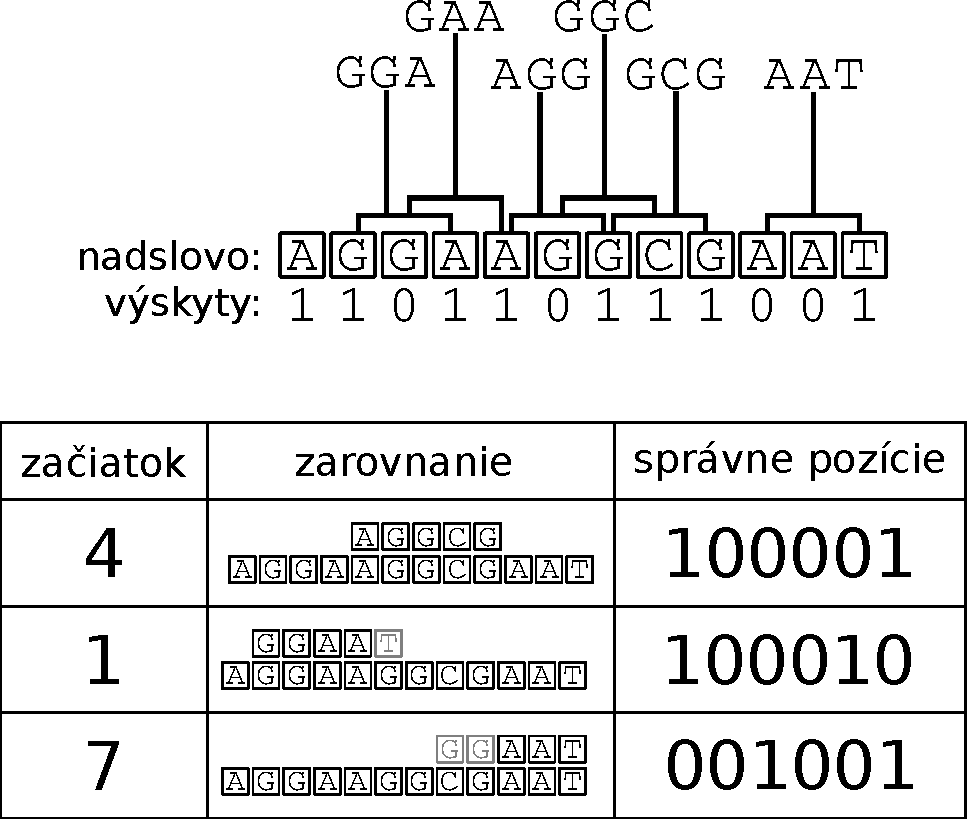
\includegraphics[width=1\textwidth]{images/zarovnanie-3-3.pdf}}

\caption[Zarovnanie a štruktúry]{Ukážkový príklad začiatkov a zodpovedajúcich úsekov v poli správnych pozícií
pre vstupné slová $\texttt{ACCGC}$ a $\texttt{GGAAT}$ s $k$-nadslovom $\texttt{AGGAAGGCGAAT}$ a poľom výskytov
$\texttt{110110111001}$, kde $\texttt{1}$ reprezentuje hodnotu $Pravda$.}

\label{obr:zar-struct}

\end{figure}


Ak chceme pre $i$-ty začiatok $z$ a pre nejaký
úsek pozícií od $x$ po $x+c$ v tomto začiatku zistiť, či je tento úsek správny,
stačí nám overiť si dve vlastnosti:
\begin{enumerate}
    \item $rank(i*(q+1) + x) \equiv 1 \pmod{2}$
    \item $rank(i*(q+1) + x) = rank(i*(q+1) + x + c)$
\end{enumerate}
Prvou z týchto požiadaviek zaručíme, že pozícia $x$ je naozaj správna, druhou
zaručíme, že medzi $x$ a $x + c$ sú tiež všetky pozície správne, keďže v nich
nenastal žiaden koniec správneho úseku.

Očakávame, že takáto reprezentácia poľa správnych pozícií bude obsahovať iba
málo hodnôt $Pravda$, na jej uloženie teda môžeme využiť vhodnú štruktúru pre
riedke polia, $sdarray$ \cite{sdarray}, opäť použijeme implementáciu z SDSL.
Na reprezentáciu poľa dĺžky $n$ s $m$ hodnotami potrebujeme $m\cdot(2 + \lceil log\frac{n}{m} \rceil )$
bitov, počítanie $rank$ nám zaberie nanajvýš $O(log \frac{n}{m}) + O(\frac{log^4 m}{log n})$
operácii, aj keď v praxi je táto operácia rýchlejšia.

Aby sme vedeli rýchlo vyhľadávať, zavedieme si ešte jedno pole, ktoré bude
obsahovať smerníky na začiatky, usporiadané podľa pozície začiatku. Pomocou
tohto poľa budeme vedieť rýchlo zistiť, ktoré začiatky za prekrývajú
s nejakým úsekom pozícií v $k$-nadslove.

Aby sme vedeli povedať, ktorému čítaniu zodpovedá nejaký začiatok, zavedieme
si nové pole pravdivostných hodnôt. Toto pole bude rovnako dlhé ako pole začiatkov
a hodnotu $Pravda$ bude mať pri prvom začiatku každého čítania. Dôležité je uvedomiť
si, že začiatky vytvárame postupne pre prvé čítanie, potom pre druhé, atď.
Pre $i$-ty začiatok zistíme, ktorému čítaniu zodpovedá, pomocou $rank(i)$ v tomto novom poli.

\subsection{Riešenie dotazu}

Pre hľadaný reťazec $r$ si najprv nájdeme, kde sú jeho výskyty v $k$-nadslove
pomocou FM-indexu. Spomedzi všetkých týchto výskytov nás budú zaujímať iba tie,
ktorých koniec má v poli výskytov hodnotu $Pravda$.

Pre každý takýto výskyt binárne vyhľadáme najmenší začiatok, ktorý sa kryje s celým
výskytom a overíme si v poli správnych pozícií, či nejde o falošný prekryv.
Ak je prekryv naozaj pravý, pridáme čítanie, ktorému zodpovedal daný začiatok,
do výsledku. Podobne ako pri počítaní výskytov budú nastávať problémy pre $r$
kratšie než $k$.

Časová zložitosť tohto dotazu závisí od vyhľadávania v FM-indexe, nájdenia
prvého začiatku a následného
kontrolovania potenciálnych začiatkov. Keďže očakávame, že v FM-indexe bude
iba málo výskytov dotazovaného reťazca a prvý potenciálny začiatok binárne
vyhľadávame, väčšina času vykonávania tohto dotazu bude plynúť z kontrolovania
potenciálnych začiatkov. Časová zložitosť kontrolovania potenciálnych začiatkov
je lineárne závislá od ich počtu.

\subsection{Redukcia počtu začiatkov}

Veľkosť všetkých týchto pomocných štruktúr a čas vykonávania
dotazu sú úzko späté s počtom začiatkov, ktoré si ukladáme. V tejto
časti si popíšeme, ako budeme ešte počas vytvárania $k$-nadslova zmenšovať
počet týchto začiatkov.

Vo výslednom korektnom slede v $k$-grafe vstupnej
množiny slov budeme preferovať, aby niektoré hrany boli použité priamo po sebe.
Pokiaľ máme napríklad pri $k = 3$ vstupné slovo \verb_AGGC_, budeme preferovať,
aby po hrane z vrchola \verb_(AG)_ do \verb_(GG)_ nasledovala hrana z \verb_GG_
do \verb_GC_. Tým dosiahneme, že vo výslednom $k$-nadslove sa bude nachádzať
podreťazec \verb_AGGC_, čiže $k$-tice \verb_AGG_ a \verb_GGC_ budú mať ten istý
začiatok.

Keďže samotné rýchle hľadanie Eulerovského ťahu v grafe sa ťažko prispôsobuje
preferovaniu nejakej následnosti hrán, zavedieme si jednoduchú
operáciu spájania hrán na grafe, ktorú budeme vykonávať ešte pred hľadaním ťahu. Pokiaľ
máme hrany $e_1 = (V_1, V_2)$ a $e_2 = (V_2, V_3)$ a preferujeme, aby $e_2$
nasledovala po $e_1$, môžeme obe hrany z grafu odstrániť a pridať namiesto nich \emph{spojenú}
hranu $e_3 = (V_1, V_3)$. Spojiť môžeme samozrejme aj viacero hrán dohromady. Pre
každú spojenú hranu si budeme pamätať postupnost pôvodných hrán, z ktorých sa
skladá.

\begin{figure}

\centerline{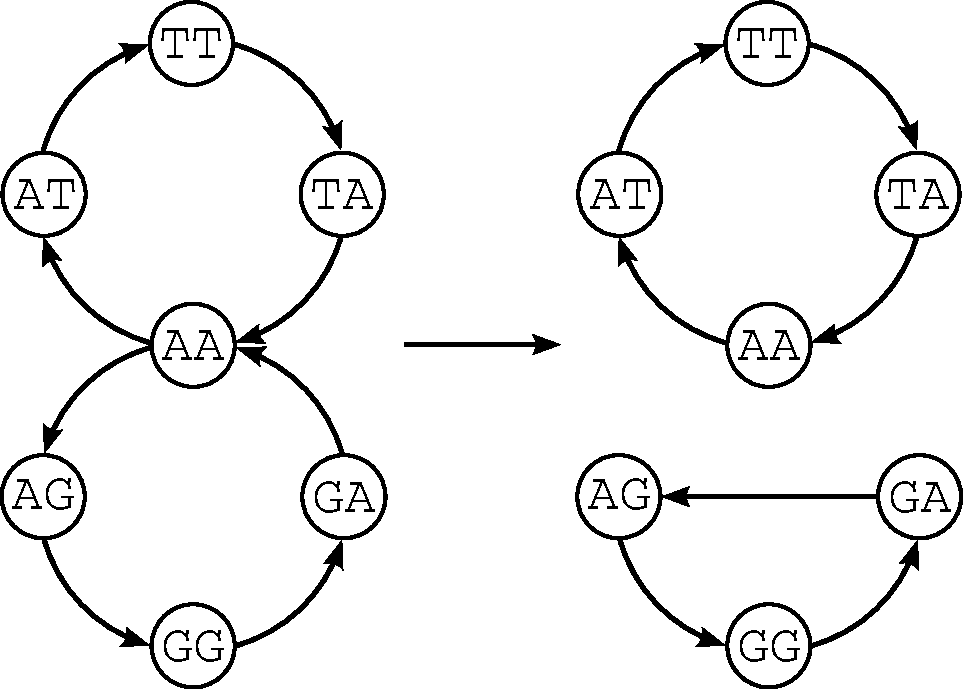
\includegraphics[width=0.7\textwidth]{images/rozpadnutie-3-3.pdf}}

\caption[Zvýšenie počtu komponentov]{Ukážkový príklad rozpadu grafu na komponenty
pri spojení hrán.}

\label{obr:rozpad}

\end{figure}

Jednou nevýhodou takejto operácie je, že môže zvýšiť počet komponentov v grafe.
Ako jednoduchý príklad môže slúžiť graf pozostávajúci z dvoch cyklov, ktoré
zdieľajú jeden vrchol $V$. Ak v jednom z týchto cyklov prepojíme hrany
prechádzajúce cez $V$, pôvodne súvislý graf sa rozpadne na dva komponenty.
Tento príklad sme znázornili na obr. \ref{obr:rozpad}.

Spájať hrany môžeme viacerými spôsobmi, niektoré z nich môžu zaručiť, že sa
nezvýši počet komponentov, niektoré môžu aj napriek zvýšeniu počtu komponentov
pospájať viacero hrán dohromady. V našej implementácii sme sa rozhodli pre druhú
z týchto možností, keďže predpokladáme, že nám takto vznikne pomerne málo nových
komponentov a za každý rozpad sa nám $k$-nadslovo predĺži najviac o $k-1$ znakov.

Základný algoritmus nadpájania hrán, ktorý používame, bude nasledovný:
\begin{enumerate}
    \item Prejdi cez všetky vstupné slová a pre každú dvojicu hrán $e_1$ a $e_2$, ktoré
          môžu ísť po sebe zisti, v koľkých vstupných slovách naozaj idú po sebe.\\
          Túto hodnotu označíme ako skóre spojenia hrán $e_1$ a $e_2$.
    \item V každom vrchole grafu nájdi párovanie hrán s najväčším súčtom skóre. Z
          párenia odstráň spojenia hrán s nulovým skóre.
    \item Spoj všetky postupnosti hrán, ktoré vznikli v predošlom kroku.
\end{enumerate}

Pri predbežných testoch tento postup naozaj počet
komponentov grafu $k$-grafu vstupných slov zvýšil iba minimálne. Tým pádom
sa nijako výrazne nezmenila dĺžka $k$-nadslova.
Počet začiatkov však klesol zhruba na polovicu.
